\section{Presentation and Discussion of Results}

As we briefly explained in section \ref{data-visualization}, the number of initial face examples is slightly greater than the number of non-face examples, so, we decided not to use accuracy as performance metric, because it becomes misleading. Instead, we used the combination of \textbf{F1 Score}, \textbf{Accuracy}, \textbf{Precision} and \textbf{Recall} to compare both models.

To clarify these concepts:

\begin{itemize} 
\item \textbf{Precision} - the fraction of correctly classified positive examples from all classified as positive.
\item \textbf{Recall} - actual positive rate of all positive examples, that is, the fraction of correctly classified examples.
\item \textbf{F1 Score} - weighted average of Precision and Recall.
\end{itemize}

Furthermore, these concepts have mathematical representations, as follows:

\begin{itemize} 
\item  \(Precision = \frac{TP}{TP+FP}\)  \\
\item  \(Recall = \frac{TP}{TP+FN}\) \\
\item  \(F1 Score = 2*\frac{Recall * Precision}{Recall + Precision}\) \\
\end{itemize}

\subsection{SVM}

After optimizing our SVM classifier, we tested it with our testing dataset. As we can see in figure \ref{fig:svm-cross-validation} previously showed, the results of both train and cross-validation phases were good, as we could find a combination of parameters where the accuracy of the model in both phases had the value of 1.

Hence, in the table \ref{table:svm-results} we can clearly see what values of \textbf{F1 Score}, \textbf{Accuracy}, \textbf{Precision} and \textbf{Recall} our model was able to achieve.

\begin{table}[H]
\centering
\caption{SVM Results}
\begin{tabular}{ccccc}
\cline{2-3}
\multicolumn{1}{l|}{}                & \multicolumn{1}{l|}{\textbf{Train \& Cross-Validation}} & \multicolumn{1}{l|}{\textbf{Test}} &  &  \\ \cline{1-3}
\multicolumn{1}{|l|}{\textbf{F1 Score}} & \multicolumn{1}{c|}{1}                     & \multicolumn{1}{c|}{0.985}                              &  &  \\ \cline{1-3}
\multicolumn{1}{|l|}{\textbf{Accuracy}} & \multicolumn{1}{c|}{1}                     & \multicolumn{1}{c|}{0.985}                              &  &  \\ \cline{1-3}
\multicolumn{1}{|l|}{\textbf{Precision}} & \multicolumn{1}{c|}{1} & \multicolumn{1}{c|}{0.985} & & \\ \cline{1-3}
\multicolumn{1}{|l|}{\textbf{Recall}} & \multicolumn{1}{c|}{1} & \multicolumn{1}{c|}{0.986} & & \\\cline{1-3} & & & & 
\end{tabular}
\label{table:svm-results}
\end{table}

As we can see, and reiterating the behaviour of our SVM classifier on both testing and cross-validation phases, we can see that all four metrics have the value of \(1\). In the testing phase, the results were not perfect, that is, the values are a little bit lower than \(1\), however, were quite good, as we were able to achieve a success rate approximately close to \(0.985\). It is necessary to remember that these results are not related to just one execution, but to \(50\) executions of the entire flow. This means that the values presented in table \ref{table:svm-results}, represent the average of each metric for the \(50\) repetitions of the entire flow (dataset splitting, training, cross-validation and testing).

Furthermore, to help us understand if the classifier was systematically incorrectly classifying one of the classes, we decided to produce the confusion matrix that can be seen in figure \ref{fig:svm-confusion-matrix}.

\begin{figure}[htbp]
\centerline{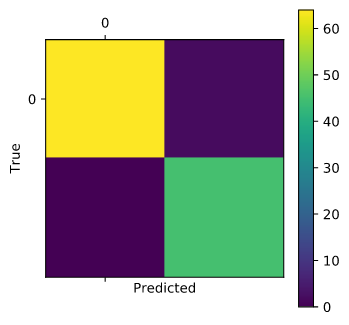
\includegraphics[width=0.65\linewidth]{images/svm_conf_matrix.png}}
\caption{SVM - Confusion Matrix}
\label{fig:svm-confusion-matrix}
\end{figure}

As we analyse the confusion matrix related to the results on the testing dataset, in figure \ref{fig:svm-confusion-matrix}, we can see that the model it's not systematically miss-classifying some of the classes, which means that our data augmentation of the dataset was able to regularize the learning process of our model. We can also see that in each class we have less than 5 examples miss-classified, which we see as positive outcome.

\subsection{NN}

To the Neural Network classifier, the adopted flow was similar to the one detailed above, that is, we optimized our NN model and then tested it on the testing dataset.

The table \ref{table:nn-results} summarizes the result values the NN model was able to achieve.

\clearpage

\begin{table}[htbp]
\centering
\caption{NN Results}
\begin{tabular}{ccccc}
\cline{2-3}
\multicolumn{1}{l|}{}                & \multicolumn{1}{l|}{\textbf{Train \& Cross-Validation}} & \multicolumn{1}{l|}{\textbf{Test}} &  &  \\ \cline{1-3}
\multicolumn{1}{|l|}{\textbf{F1 Score}} & \multicolumn{1}{c|}{1}                     & \multicolumn{1}{c|}{0.973}                              &  &  \\ \cline{1-3}
\multicolumn{1}{|l|}{\textbf{Accuracy}} & \multicolumn{1}{c|}{1}                     & \multicolumn{1}{c|}{0.973}                              &  &  \\ \cline{1-3}
\multicolumn{1}{|l|}{\textbf{Precision}} & \multicolumn{1}{c|}{1} & \multicolumn{1}{c|}{0.974} & & \\ \cline{1-3}
\multicolumn{1}{|l|}{\textbf{Recall}} & \multicolumn{1}{c|}{1} & \multicolumn{1}{c|}{0.974} & & \\\cline{1-3} & & & & 
\end{tabular}
\label{table:nn-results}
\end{table}

As can be seen in table \ref{table:nn-results}, as in our SVM model, for training and cross-validation phases, the model achieve the value of \(1\) to every metric, but for the testing phase, our NN model performed worse than our SVM model, achieving the average values of \(0.97\) to each evaluation metric. 

Moreover, we also produced the confusion matrix to this model, as can be seen in figure \ref{fig:nn-confusion-matrix}. As in the SVM model, our NN classifier it's not systematically miss-classifying the examples, which confirms the conclusion we stated above about the data augmentation process. As in our SVM model, we can see that the miss-classified examples were also on a reduced number, although a little higher than in the SVM model. With this, we were able to conclude that neither of the models had systematic miss-classification problems and that our NN model was not able to generalize its predictions as much as the SVM classifier.

\begin{figure}[htbp]
\centerline{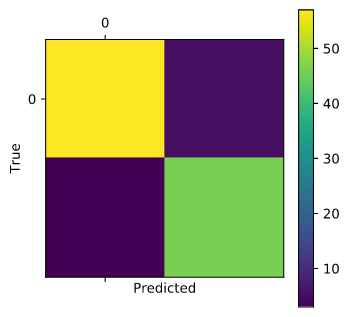
\includegraphics[width=0.65\linewidth]{images/nn_conf_matrix.png}}
\caption{NN - Confusion Matrix}
\label{fig:nn-confusion-matrix}
\end{figure}

The purpose of this paper was always to compare the two models against each other. However, we always thought the NN model would be better than the SVM model, even if by a little range. After these results, we came to the conclusion that this could be related with a number of causes:

\begin{itemize} 
\item The dataset size that was not that big, and can harm the learning process of the NN model, that ends up needing more data than the SVM model.
\item The feature extractor function: both models used the same feature extraction function (HOG) as a mean to achieve common ground and a true state of comparison, and that could indeed be one of the reasons, since other feature extractors, such as \textit{Fast Gabor Filtering}, produce better results on Neural Network models.
\end{itemize}

These possibilities will be further detailed in section \ref{novelty}.

\subsection{External Test Examples}

Finally, after testing our two models with the testing dataset, we decided to test both models with external images that weren't part of the original dataset. Thus, we slightly modified how we processed the images and its predictions so we could test an example with multiple faces and a more complex context to assert how our models would handle that test case.

As we can see in figures \ref{fig:svm-family-result} and \ref{fig:nn-family-result}, both models successfully identified all the existent faces in the images and both models produced instances of false positive results. We can also see that the NN model produced more false positives (it produced three false positives in the testing image) than the SVM model, that only produced one. This does not come as a surprise, because we already saw that our SVM model produces better results than our NN model.

\begin{figure}[htbp]
\centerline{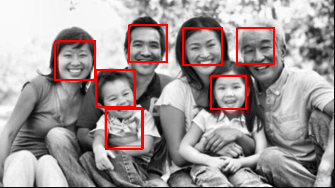
\includegraphics[width=1\linewidth]{images/svm_persons.png}}
\caption{SVM - Family External Image Test Result}
\label{fig:svm-family-result}
\end{figure}

\begin{figure}[htbp]
\centerline{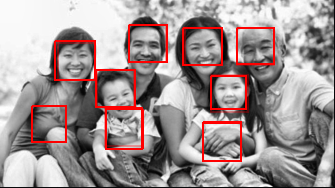
\includegraphics[width=1\linewidth]{images/nn_persons.png}}
\caption{NN - Family External Image Test Result}
\label{fig:nn-family-result}
\end{figure}

With this external test image, we were asserted that both models were able to correctly detect all existent faces, and that both had problems with false positives, which was expected as none of our models produced result scores of approximately \(1\) in the testing phase.